\documentclass{report}

%packages
\usepackage[utf8]{inputenc}
\usepackage{listings}
\usepackage{courier}
\usepackage{lipsum}
\usepackage{minted}
\usepackage{tabu}
\usepackage{graphicx}

\graphicspath{ {screenshots/} }

\title{Programming Coursework Report}
\author{Quinn Stevens}
\date{June 2017}

\begin{document}
\tabulinesep=1.2mm
\maketitle

\tableofcontents

    \part{Quiz Game}
    \chapter{Testing Plan}
    
    \begin{center}
      \begin{tabu} {|X[c]|X[c]|X[c]|X[c]|X[c]|}
        \hline
        Environment & Action & Expected Result & Actual Result & Proof\\
        \hline
        Program Closed & Run Program & Main Menu form opens & Main Menu form opened & see screenshot \ref{fig:screenshot01}\\
        \hline
        Main Menu & Click 'Quit' Button & Program closes & Program closed & see screenshot \ref{fig:screenshot02}\\
        \hline
        Main Menu & Click 'Easy' Button & Asks first easy question & Asked first easy question & see screenshot \ref{fig:screenshot03}\\
        \hline
        Quiz & Click radio button & Radio button selected & Radio button selected & see screenshot \ref{fig:screenshot04}\\
        \hline
        Quiz & Click Answer while radio button selected & Ask next question & Asked next question & see screenshot \ref{fig:screenshot05} \\
        \hline
        Quiz & Click Answer while radio button not selected & Ask next question & Asked next question & see screenshot \ref{fig:screenshot06} \\
        \hline
        Quiz & Click Skip & Ask Next Question & Asked next question & see screenshot \ref{fig:screenshot07}\\
        \hline
      \end{tabu}
    \end{center}
    
    \chapter{Testing Screenshots}
    
    \begin{figure}[H]
        \centering
        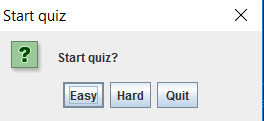
\includegraphics{Screenshot01}
        \caption{Screenshot 01}
        \label{fig:screenshot01}
    \end{figure}
    
    \begin{figure}
        \centering
        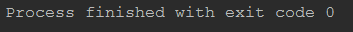
\includegraphics{Screenshot02}
        \caption{Screenshot 02}
        \label{fig:screenshot02}
    \end{figure}
    
    \begin{figure}
        \centering
        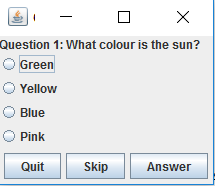
\includegraphics{Screenshot03}
        \caption{Screenshot 03}
        \label{fig:screenshot03}
    \end{figure}
    
    \begin{figure}
        \centering
        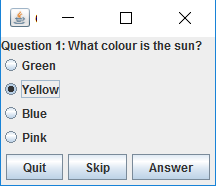
\includegraphics{Screenshot04}
        \caption{Screenshot 04}
        \label{fig:screenshot04}
    \end{figure}

    \begin{figure}
        \centering
        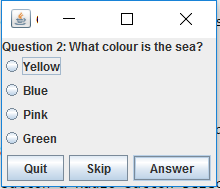
\includegraphics{Screenshot05}
        \caption{Screenshot 05}
        \label{fig:screenshot05}
    \end{figure}
    
    \begin{figure}
        \centering
        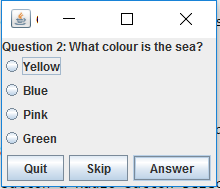
\includegraphics{Screenshot06}
        \caption{Screenshot 06}
        \label{fig:screenshot06}
    \end{figure}
    
    \begin{figure}
        \centering
        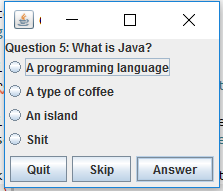
\includegraphics{Screenshot07}
        \caption{Screenshot 07}
        \label{fig:screenshot07}
    \end{figure}
    
    \chapter{Critical Analysis}
        \section{Strengths}
        \begin{itemize}
            \item blah
        \end{itemize}
        
        \section{Weaknesses}
        \begin{itemize}
            \item blah
        \end{itemize}
        
        \section{Suggested Enhancements}
    
    \chapter{Source Code}

\addcontentsline{toc}{chapter}{Appendix I: Banking Program}
\chapter*{Appendix I: Banking Program}
\section{Source Code}
\section{Output}
\end{document}
